\section{Module 4: Lecture 2\\Defining the Laplace Transform and the Z Transform}


\subsection{Introduction}
In the previous lectures you were introduced to the basic idea of extending the definition of the Fourier Transform to capture the unstable signals. It also exposed you to the definition of the \textit{Z transform} for Discrete Time Fourier Transform. In this lecture, you will be introduced to \textit{Laplace Transform} on similar motivation of the Continuous case.\\
Also, throughout the subsequent lecture we will follow the convention that the Laplace transform of $x(t)$ will be denoted $X(s)$, and the region of convergence by $R_X$. And this relation is shown by \\
Laplace transform of $x(t)$ : 
$x(t) \xrightarrow{\ \mathcal{L}\ } X(s)\ ;\ R_X $. \\
Also, Fourier transform of $x(t)$ : 
$x(t) \xrightarrow{\ \mathcal{F}\ } X(j\Omega)\ ;\ R_X $. \\ 
and Z-transform of $x(t)$ :
$x[n] \xrightarrow{\ z\ } X(z)\ ;\ R_X$

\subsection{Laplace Transform}
Consider the input $x(t) = e^{t}u(t)$. Notice that this is an exponentially growing unstable signal. As per our earlier discussion, we need to capture this growing sequence and take its Fourier Transform. For this, we will need to multiply it by a decaying exponential, let's say $e^{-\sigma t}$. Now, if we take the Fourier Transform of $x(t)e^{-\sigma t}$
\[
	X(\sigma + j\Omega) = \int_{-\infty}^{\infty}{x(t)e^{-\sigma t}e^{-j\Omega t}dt}
\]\[
	 = \int_{0}^{\infty}{e^{t}e^{-\sigma t}e^{-j\Omega t}dt}
\]\[
	 = \int_{0}^{\infty}{e^{(1-\sigma)t}e^{-j\Omega t}dt}
\]
Asking when the above Fourier Transform $X(s)$ will exist, is equivalent to asking when will the above integral converge and what are the conditions on $\sigma$ and $\Omega$.\\
Note that it will only be the $e^{(1-\sigma)t}$ which would contribute to the convergence as the other factor $e^{-j\Omega t}$ has magnitude 1 and contributes only in the phase part. Thus, $e^{(1-\sigma)t}$ needs to be a decaying exponential. It should be a negative power of $e$ which would happen if $(1-\sigma) < 0$ which implies that $\sigma > 1$. If we consider $\sigma + j\Omega = s$ where s is a complex constant with $\Re(s) = \sigma$ and $\Im(s) = \Omega$ then the Fourier Transform becomes 
\[
	X(s) = \int_{-\infty}^{\infty}{x(t)e^{-st}dt}
\]
In our considered example (for $\sigma > 1$ or $\Re(s) >1$),
\[
	X(s) = \int_{0}^{\infty}{e^{(1-\sigma)t}e^{-j\Omega t}dt}
\]\[
	 = \int_{0}^{\infty}{e^{t}e^{-st}dt}
\]\[
	 = \int_{0}^{\infty}{e^{(1-s)t}dt}
\]\[
	 = \frac{1}{(1-s)}e^{(1-s)t}\Big|_0^{\infty}
\]\[
	\mathbf{X(s) = \frac{1}{(s - 1)}}
\]
The region in the complex $s$ plane in which the above formulation exists is known as the Region Of Convergence of the \textit{Laplace Transform} which can be graphically shown by the figure below.
\begin{figure}[h!]
\begin{center}
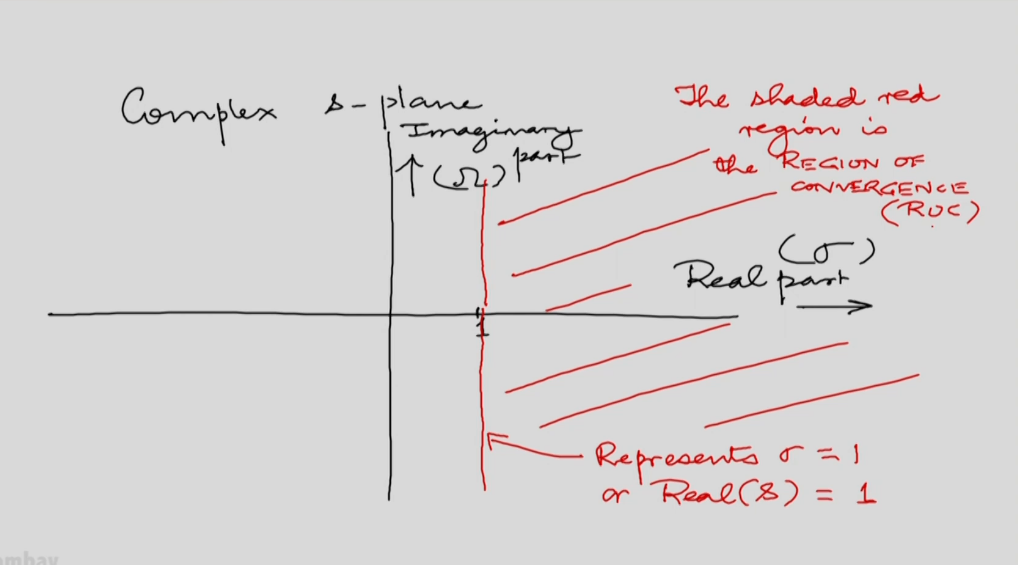
\includegraphics[width=15cm]{2_fig_1.png}
\end{center}
\caption{Region of convergence $R_X$ for the input  $x(t) = e^{t}u(t)$}
\end{figure}\\
Now consider $x_1(t) = -e^{t}u(-t)$ which is the same exponential signal on the negative half in time domain.
\[
	X_1(s) = \int_{-\infty}^{\infty}{x_1(t)e^{-st}dt}
\]\[
	 = \int_{-\infty}^{0}{-e^{t}e^{-st} dt}
\]\[
	 = \int_{-\infty}^{0}{-e^{(1-s)t} dt}
\]\[
	 = \frac{-1}{(1 - s)}e^{(1-s)t}\Big|_{-\infty}^{0}
\]\[
	\mathbf{X_1(s) = \frac{1}{(s - 1)}}
\]
But observe that during the second last step we need to realise that for the definite integral to exist, we need $e^{(1-s)t}$ to go down to 0 as t tends to ${-\infty}$. Thus we have $\Re(1-s) > 0$ which implies $\Re(s) < 1$. \\
Thus, Laplace Transform of $x_1(t) = -e^{t}u(-t)$ is $\mathbf{X_1(s) = \frac{1}{(s - 1)}}$ with $\ R_X: \Re(s) < 1$ or $\sigma < 1$. It is exactly the complement graph of that shown in Figure 1.

\subsection{Significance of the Region of Convergence}
We have seen that the \emph{expression} for the Laplace transform of $x(t)$ and $x_1(t)$ come out to be exactly the same, even though they are different signals. This indicates that the Laplace Transform is not only the expression in terms of $s$ but also the Region of Convergence(ROC). If we don't consider ROC also, we might be looking at a wrong expression!
\[
e^{t}u(t) \xrightarrow{\ \mathcal{L}\ } \frac{1}{(s - 1)}\ ;\ Re(s) > 1. \]\[
-e^{t}u(-t) \xrightarrow{\ \mathcal{L}\ } \frac{1}{(s - 1)}\ ;\ Re(s) < 1. 
\]
We start by observing that the Laplace Transform of both the signals is the same and the only difference is the ROC which are mutually exclusive regions. For a signal to apriori have a Fourier Transform we need to have $\Re(s) = 0$ i.e. $\sigma = 0$ contained in the ROC. This is because if $\sigma=0$, then $s=j\Omega$, and the expression for the Laplace transform just reduces to that of the Fourier transform. Thus, if the Laplace transform does not exist for $\sigma=0$, that means that the Fourier transform too does not exist. Thus we conclude that the signal with $\Re(s)=0$ in its region of convergence does a priori have a Fourier Transform but for the other, we will have to hold it down so that the Fourier Transform exists.
In our example, $x_1(t)$ contains $\Re(s)=0$ in its ROC, and hence has a Fourier transform, whereas $x(t)$ doesn't.
To have a comparative picture of the two discussed signals, observe the Figure 2.
\begin{figure}[h!]
\begin{center}
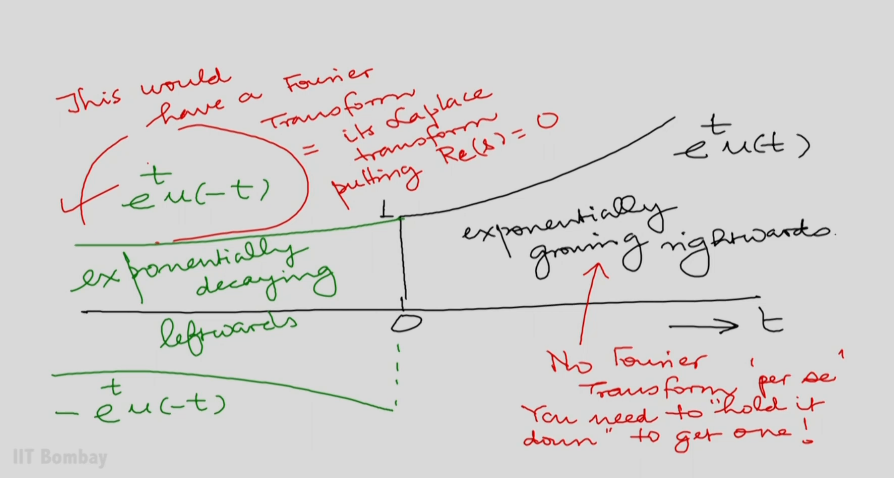
\includegraphics[width=15cm]{2_fig_2.png}
\end{center}
\caption{Region of convergence $R_X$ for the input  $x(t) = e^{t}u(t)$}
\end{figure}

%\subsection{Comparison between Laplace and Fourier Transforms}
%The Laplace transform also bears a straightforward relationship to %the Fourier transform when the complex variables is not purely %imaginary. To see this relationship, consider the Laplace Transform %$X(s)$ with s expressed as $s = (\sigma + j\Omega)$, so that
%\[
%	X(\sigma + j\Omega) = \int_{-\infty}^{\infty}{x(t)e^{-(\sigma + j\Omega) t}dt}
%\]\[
%	X(\sigma + j\Omega) = \int_{-\infty}^{\infty}{[x(t)e^{-\sigma t}]e^{-j\Omega t}dt}
%\]
%We recognize the second equation as the Fourier transform of %$x(t)e^{-\sigma t}$, that is, the Laplace transform of $x(t)$ can be %interpreted as the Fourier transform of $x(t)$ after multiplication %by a real exponential signal. The real exponential $e^{-\sigma t}$ %may be decaying or growing in time, depending on whether $\sigma$ is %positive or negative.

\subsection{Z Transform Equivalent Summary}
The Z-transform of a sequence $x[n]$ is given by $X(z)$
\[
X(z) = \sum_{n=-\infty}^{\infty}{x[n]z^{-n}}
\]
For example if $x[n] = 3^{n}u[n]$
\[
X(z) = \sum_{n=-\infty}^{\infty}{3^{n}u[n]z^{-n}}
\]\[
X(z) = \sum_{n=0}^{\infty}{{(\frac{3}{z}})^{n}}
\]\[
	\mathbf{X(z) = \frac{z}{z-3}}
\]

With the Region of Convergence :
\[
	\mathbf{R_X : |z| > 3}
\]
\begin{figure}[h!]
\begin{center}
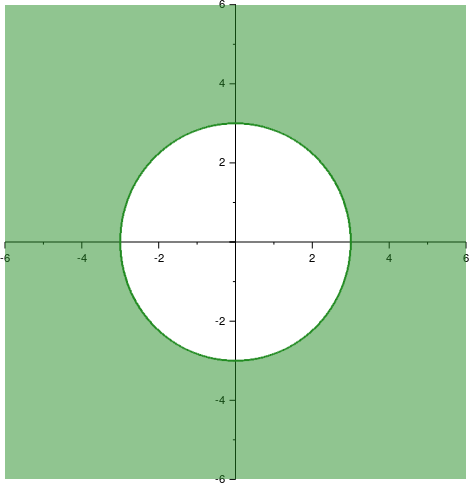
\includegraphics[width=5cm]{plot_2.png}
\end{center}
\caption{Region of convergence $R_X$ for the input  $x[n] = 3^{n}u[n]$}
\end{figure}

\subsection{Conclusion}
In this lecture, we looked at the definition of \textit{Laplace transform} with some basic examples. It also invoked the importance of the Region of Convergence in Laplace Transforms and its eqivalence in Z-Transforms. In the subsequent lectures we will go about solving some examples of both Laplace and Z-transforms.







                



                     
